\documentclass[11pt]{article}
\usepackage{tutorial-students}
\usepackage{tikz}
\usepackage{tkz-graph}
\usepackage{hyperref}

\newcommand{\fillinMCmath}[1]{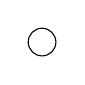
\begin{tikzpicture}\draw circle [radius=0.5em];\end{tikzpicture}\ #1}
\newcommand{\fillinMCmathsoln}[1]{
\begin{tikzpicture}\draw[black, fill=blue] circle [radius=0.5em];\end{tikzpicture}\ #1}

\newcommand{\Cats}{{\cal C}}

\author{}
\date{}
\begin{document}

\title{CPSC 320 2021W1: Assignment 3}

\maketitle
\vspace{-0.5in}

This assignment is due on \textbf{Wednesday, Oct 27 at 10pm Vancouver time} on Gradescope. Assignments submitted within 24 hours after the deadline will be accepted, but a penalty of 15\% will be applied. Please follow the guidelines provided in Assignment 1.

All the submission and formatting rules for Assignment~1 apply to
this assignment as well.  For drawings of graphs, however, we will permit
pictures of hand-drawn graphs included in your PDF submission, as we did
with pseudocode on the last assignment, as long as they are clear and
easy-to-mark.

%------------------------------------------------------------------------------
\section{List of names of group members (as listed on Canvas)}

Provide the list here. This is worth 1 mark. Include student numbers
as a secondary failsafe if you wish.

\begin{soln}
Mathew Balsdon 21041694 \\
Michael Woolsey 87234621
\end{soln}

\section{Statement on collaboration and use of resources}
To develop good practices in doing homeworks,
citing resources and acknowledging input from others, please complete the following.
This question is worth 2 marks.

\begin{enumerate}
\item All group members have read and followed the guidelines for groupwork
on assignments given on the website (see \url{https://www.students.cs.ubc.ca/~cs-320/2021S2/coursework.html}, under Assignments).

\fillinMCmathsoln{Yes} \hspace{.5in} \fillinMCmath{No}

\item We used the following resources (list books, online sources, etc. that you consulted):
\begin{soln}
We used these guides to help us understand how greedy proofs should be structured:

\url{https://web.stanford.edu/class/archive/cs/cs161/cs161.1138/handouts/120\%20Guide\%20to\%20Greedy\%20Algorithms.pdf}

\url{http://www.cs.cornell.edu/courses/cs482/2004su/handouts/greedy_ahead.pdf}
\end{soln}
\item One or more of us consulted with course staff during office hours.

\fillinMCmath{Yes} \hspace{.5in} \fillinMCmathsoln{No}

\item One or more of us collaborated with other CPSC 320 students; none of us took
      written notes during our consultations and we took at least a half-hour break afterwards.

\fillinMCmath{Yes} \hspace{.5in} \fillinMCmathsoln{No}

      If yes, please list their name(s) here:


\item One or more of us collaborated with or consulted others outside of CPSC 320; none of us took written notes during our consultations and we took at least a half-hour break afterwards.

\fillinMCmath{Yes} \hspace{.5in} \fillinMCmathsoln{No}

      If yes, please list their name(s) here:

\end{enumerate}
\newpage

\section{Max-Min Clustering}

Suppose that we change the goal of the photo categorization problem in the worksheet to {\em maximize the minimum intra-cluster edge similarity}. We call this Max-Min categorization. (In contrast, the goal in the worksheet was to minimize the maximum inter-category edge similarity.)

\begin{enumerate}
\item (1 mark)
  For the 4-node example from the worksheet, shown below, and $c=2$, list all of the optimal Max-Min categorizations. No justification needed.

  \vspace{.1in}

  \begin{center}
\includegraphics[width=3.5in]{clustering-example.png}
  \end{center}
  \vspace{.1in}
\begin{soln}
$\{\{3,1\},\{2,4\}\}$
\end{soln}

\item (1 mark)
  Here is a greedy algorithm that produces a categorization:


  \begin{algorithmic}[1]
\Function{New-Clustering-Algorithm}{$n,E,c$}
\State $\triangleright$ $n \ge 1$ is the number of photos
\State $\triangleright$ $E$ is a set of edges of the form $(p,p',s)$,
where $s$ is the similarity of $p$ and $p'$
\State $\triangleright$ $c$ is the number of categories, $1 \le c  \le n$
\State create a list of the edges of $E$, in increasing order by similarity
\State let $\Cats$ be the categorization with all photos in one category

\State Num-$\Cats \gets 1$  $\triangleright$ Initial number of categories
\While{Num-$\Cats < c$}
   \State remove the lowest-similarity edge $(p,p',s)$ from the list
   \If{$p$ and $p'$ are in the same category, say $S$, of $\Cats$}
      \State $\triangleright$ split $S$ into two new categories $T$ and $T'$ as follows:
      \State put $p$ in $T$
      \State put $p'$ in $T'$
      \For{each remaining $p''$ in $S$}
         \State  put $p''$ in $T$ if $p''$ is more similar to $p$ than $p'$
         \State  put $p''$ in $T'$ otherwise
         \EndFor
      \State $\triangleright$ now $S$ is replaced by $T$ and $T'$ in $\Cats$
      \State Num-$\Cats$  $\gets$ Num-$\Cats + 1$
   \EndIf
\EndWhile
\State \Return $\Cats$
\EndFunction      
\end{algorithmic}

What categorization does New-Clustering-Algorithm produce on the 4-node example given at the start of this question? No justification needed.\\
\begin{soln}
$\{\{3,1\},\{2,4\}\}$
\end{soln}

\item (4 marks)
  Let $(n,E,c)$ be an input where all edges have distinct similarities, and $c \ge 2$. Suppose that $(p,p',s)$ is the edge removed in the first iteration of the {\bf while} loop. In an {\em optimal} Max-Min categorization, must $p$ and $p'$ be in distinct categories?

 \begin{soln}
 We know that in the first iteration, the two nodes, $p$ and $p'$ with the lowest similarity will for sure be separated into two categories, by lines 9-13. The only way that they could be placed back into the same category is if lines 15 and 16 ran such that $p$ was more similar to $p'$ over some other node $q$, or if $p'$ was more similar to $p$ over some other node $q'$. However, this could never happen because $p$ and $p'$ share the least similarity out of all nodes, since similarities are distinct and the first iteration splits the two least similar nodes. Therefore, it must be the case that the optimal Max-Min categorization would have $p$ and $p'$ in distinct categories.
 \end{soln}

\item (3 marks)
  Let $E'$ be the set of all edges removed from the list, over all iterations of the {\bf while} loop of New-Clustering-Algorithm, and let $C^G$ be the categorization returned by the algorithm. Which statement is true? Choose one, and justify your answer.

  \fillinMCmathsoln{All edges of $E'$ must be inter-category edges of $C^G$.}

  \fillinMCmath{All edges of $E'$ must be intra-category edges of $C^G$.}

  \fillinMCmath{Edges of $E'$ could be both intra-category and inter-category edges of $C^G$.}
  
  \begin{soln}
  For an edge, $e=(p,p',s)$, that we remove in line 9. There are two possibilities when we reach line 10, either:
  p and p' are in the same category, in which case we will split them into two different groups (and become inter-category). 
  Or, p and p' are already inter-category. This means that for every e in E', the edge must be inter-category.
  \end{soln}
  
  
\item
  (3 marks)
Describe a 4-node instance of the Photo Categorization problem, on which New-Clustering-Algorithm is incorrect. That is, New-Clustering-Algorithm produces a solution that does {\em not} maximize the minimum intra-cluster edge similarity on your instance.


\begin{soln}

\includegraphics[width=300px]{unknown.png}\\
Following the steps in the diagram will result in a final grouping $\{\{1 \}, \{ 2\},\{3,4 \}\}$ (min intra-cluster edge = 0)  that does not equal the optimal solution: $\{\{1,4 \}, \{ 2\},\{3 \}\}$ (min intra-cluster edge = 1).
\end{soln}

  \end{enumerate}
\newpage
\section{Spend those coupons!}
Every day, you go to the restaurant next door to buy your lunch. The restaurant has a coupon program for loyal customers, and you have accumulated $n$ coupons, each with their own discount value and expiry date. You cannot use more than one coupon per day, which means that you may not have enough days to use all the coupons before each of their expiry dates have passed. Your goal is to find a subset (not necessarily a proper subset) of coupons that
\begin{enumerate}
    \item[(a)] is “usable” - it is possible to use each coupon in the set before its expiry date, and 
    \item[(b)] maximizes your total savings, that is the sum of the discount values of each coupon used. 
\end{enumerate}

Each coupon $i$ is represented as a tuple, $(d_i, e_i)$, where $d_i$ is the discount value and $e_i$ is the expiry date. The expiry dates are positive integers, so if $e_i=k$, coupon $i$ must be used on or before day $k$, assuming we start at day 1. For example, suppose you have the following set of $n = 5$ coupons:
\begin{table}[h]
    \centering
    \begin{tabular}{l|ll} 
    $i$ & $d_i$ & $e_i$ \\ \hline
    1 & 3 & 2   \\
    2 & 4 & 3   \\
    3 & 1 & 1   \\
    4 & 6 & 2   \\
    5 & 5 & 5   \\
    \end{tabular}
\end{table}

There is no particular order to the coupons. Here are some examples of usable subsets of coupons and their corresponding total savings. 
\begin{itemize}
    \item[] $\{ 3, 1, 2, 5\}$, with a total savings value of 1+3+4+5=13
    \item[] $\{ 3, 4, 2, 5\}$, with a total savings value of 1+6+4+5=16
    \item[] $\{ 4, 1, 2, 5\}$, with a total savings value of 6+3+4+5=18
\end{itemize}
The complete set of coupons $S = \{1,2,3,4,5\}$ is not usable, since it is not possible to use coupons 1, 2, and 3 within their respective expiry dates. For this particular instance, 18 is indeed the optimal total savings. 

\begin{enumerate}
    \item (3 marks) Consider the following greedy algorithm. While it does always return a usable set of coupons, it does not always find an optimal set of coupons. Give a counterexample to show this. 
    
    \begin{algorithmic}[1]
        \Procedure{$\textsc{SuboptimalGreedy}$}{$D$,$E$,$n$}
            \State{$S \leftarrow \{\}$ }
            \For{$k$ from 1 to $n$}
                \If{there is a coupon not in $S$ with $e_c \geq k$}
                    \State choose such a coupon $c$ that maximizes $d_c$
                    \State add $c$ to $S$
                \EndIf
            \EndFor
            \State \Return $S$
        \EndProcedure
    \end{algorithmic}
    
    \begin{soln}
    For the following table:
    \begin{table}[h]
    \centering
    \begin{tabular}{l|ll} 
    $i$ & $d_i$ & $e_i$ \\ \hline
    1 & 1 & 1 \\
    2 & 2 & 2 \\
    \end{tabular}
    \end{table}
    \\The algorithm will not produce the optimal solution (\{1,2\}). In the first iteration, both coupons will be eligible however line 5 mandates that coupon $i=2$ will be chosen over $i=1$ since $d_2=2 \geq d_1=1$. In the next iteration $k=2$, coupon $i=1$ will not be able to be chosen since $e_1=1 \ngeq 2$, leaving us with \{2\} instead of the optimal solution.
    \end{soln}
    
    
    \clearpage
    
    \item (4 marks) Now consider the following greedy algorithm. 
    
    \begin{algorithmic}[1]
        \Procedure{$\textsc{OptimalGreedy}$}{$D$,$E$,$n$}
            \State $S \leftarrow \{1,2,\dots,n\}$ 
            \State sort arrays $D$ and $E$ in order of increasing $E[i]$
            \State $k \leftarrow 1$
            \For{$i$ from 1 to $n$}
                \If{$E[i] < k$}
                    \State let $c$ be a coupon that minimizes $d_c$ among all $c\in S$ such that $e_c < k$ 
                    \State remove $c$ from $S$
                \Else
                    \State $k \leftarrow k + 1$
                \EndIf
            \EndFor
            \State \Return $S$
        \EndProcedure
    \end{algorithmic}
    Let $S_j$ denote the set $S$ after $j$ iterations of the while loop. Using induction on $j$, prove that the algorithm returns an optimal set of coupons. 
    
    \begin{soln}
    
    \textbf{Base case:} \\
    For iteration $j=1$, we enter the loop with $i=1, k=1$. $E[1] \nleq 0$ since that would mean it's already expired, therefore $0 < E[1] \nless k=1$ meaning line 9-10 runs in the if-else statement. This doesn't modify our set $S_1$, which contains all coupons $\{1, 2, ... , n\}$ and therefore an optimal subset of coupons. \\
    
    \textbf{Inductive step:} \\
    Assume $S_j$ contains an optimal subset of coupons $\{1, 2, ... , m\}$. \\
    
    \textbf{Inductive hypothesis:} \\
    For any iteration $j+1$, the set $S_{j+1}$ contains an optimal subset of coupons. \\
    
    At the start of line 6 of iteration $j+1$, we know our list $S_j$ contains an optimal subset as per our assumption. From here, there are two possible cases:\\
    
    $E[i] < k$: \\
    In this case, we know $ E[i]$ must have the same value as $ E[i-1]$ (since k increases by 1s only when $E[i]\geq k$, and E is sorted increasingly). This means that we will not be able to use every coupon from $E[1..i]$; there aren't enough days $k$ to use all coupons $E[1..i]$. In line 7, we select the coupon from this set with the smallest discount, and then remove it from S. $S_{j+1}$ will still be optimal after this, as we couldn't use all $k$ coupons in the optimal case and we removed the least valuable one in this iteration. \\
    
    $E[i] \nless k$:\\
    Here, we simply increment k without any changes to S, therefore $S_{j+1} = S_j$, which from our assumption contains the optimal set. \\
    
    Both cases result in $S_{j+1}$ having an optimal subset, therefore $S_{j+1}$ has an optimal subset.
    \end{soln}
    
\end{enumerate}

\clearpage

\section{Client satisfaction}

You are a contractor, and you have committed to a full schedule through the summer months. You have signed a contract with $n$ different clients, and you have guaranteed each client that their project will be complete within $n$ weeks. Each project will take you exactly one week so you can meet all of your deadlines. You must decide the order in which to complete the projects. 

All of your clients would prefer to have their project completed earlier rather than later. The earlier you complete a project for a client, the more satisfied that client is. More precisely, if you complete the project for client $i$ at the end of week $j$, then client $i$'s satisfaction is $s_i = n - j$.

Some clients are more important to you than others (perhaps some are paying you more, or other are more loyal). To quantify this, you assign each client $i$ a weight, $w_i$. You want to schedule your clients across the $n$ weeks such that you maximize the weighted sum of satisfaction, that is $\sum_{1 \le i \le n} w_i s_i$.

The following greedy strategy finds an optimal ordering of clients:
Complete the projects in decreasing order of $w_i$.

\begin{enumerate}
    \item (4 marks)
    Use an exchange argument to show that this greedy strategy yields an optimal schedule. 
    
    \begin{soln}
    Let $A$ be an ordering of clients produced by our greedy strategy, and assume $O$ is an optimal ordering of clients where $A \neq O$.
    
    Our solution is such that if client $i$ comes before client $j$, then $w_i > w_j$. Since $A \neq O$, the optimal solution $O$ must contain an inversion, namely that client $j$ comes before client $i$.
    
    We claim that by swapping client $j$ and $i$ in $O$, then $O$ will improve, contradicting that it was optimal. We also show that this swap makes $O$ closer to $A$. Therefore, success in showing this shows that our algorithm is the correct one.
    
    Our weighted sum of satisfaction for $O$ before swapping is equal to $WSS_1 = s_1w_1 + s_2w_2 + ... + s_jw_j + s_iw_i + ... + s_nw_n$. If we swap client $j$ and client $i$, then $s_j$ becomes what $s_i$ was previously, and $s_i$ becomes what $s_j$ was previously, since one takes a week longer and one takes a week less, so these values stay the same in our weighted sum of satisfaction after swapping. What does change are the weights. We end up with $WSS_2 = s_1w_1 + s_2w_2 + ... + s_jw_i + s_iw_j + ... + s_nw_n$. We know that $s_j > s_i$ by definition, and we also know that $w_i > w_j$ from assumption, therefore $WSS_2 > WSS_1$, which contradicts that $O$ was optimal. Furthermore, $O$ now has client $i$ and $j$ in the same place as $A$, meaning $O$ is closer to $A$, so proving that if we were to continue to do these swaps, we would result in $A$, proving that $A$ is an optimal algorithm.
    \end{soln}
    
  \item \label{variant}
    (3 marks) Instead of assuming that each job takes exactly 1 week, suppose that it takes $t_i$ weeks to complete the job $i$ (each $t_i$ must be greater than 0, though it is not necessarily an integer). You can assume that $\sum_{1\le i \le n} t_i = n$. Again, you want to maximize the weighted sum of satisfaction, that is $\sum_{1 \le i \le n} w_i s_i$, where $s_i = n - c_i$, and $c_i$ is the time of completion of the project. For example, if project $i$ is completed first, then $c_i = t_i$. If project $i'$ is completed second (after project $i$), then $c_i = t_i + t_{i'}$. 
    
Find a counterexample to show that the greedy strategy of
completing the projects in decreasing order of $w_i$ is not
optimal for this variant of the problem.\\
\includegraphics[width=445px]{theuhhhq52.png}
  \item (5 marks)
    Describe a different greedy strategy that is optimal
    on the problem variant described in part \ref{variant}, and show
    that your strategy is optimal.
    
    \begin{soln}
    The greedy strategy to use is: complete the projects in decreasing order of $w_i/t_i$
    
    Let $A$ be an ordering of clients produced by our greedy strategy, and assume $O$ is some optimal ordering of clients.
    
    Let $A_j$ be the result of our algorithm after doing $j$ jobs, and $O_j$ the result of that optimal algorithm after $j$ jobs. We will also define $WSS(X_j)$ to be the weighted sum of satisfaction for algorithm $X$ after $j$ jobs. 
    
    \textbf{Base case:} $j=1$. For WSS at j=1, it will be equal to $w_1*(n-t_1) = w_1 n - w_1 t_1$. What would maximize this quantity is to choose the one with the highest ratio of $w_1/t_1$, since then the term we subtract will be minimized while maximizing the positive term. So, we know that $A_1$ is optimal, so it must be the case that $WSS(A_1) \leq WSS(O_1)$
    
    For $j>1$, assume $A_{j-1}$ is optimal, and we will prove $A_j$ is optimal. From this, we know that $WSS(A_{j-1}) \leq WSS(O_{j-1})$. We know the term added at $A_j$ will be $w_j (n - (\sum_{1 \le i \le j} t_i) + t_j)$. Here, we will pick job $j$ which maximizes $w_j/t_j$, which makes sense, as this ratio is equivalent to saying "pick the job with the most value per unit of time", meaning that this option of j is optimal, implying that at least $WSS(A_{j}) \leq WSS(O_{j})$.
    
    Since we proved that for any value of $j>1$, $WSS(A_{j}) \leq WSS(O_{j})$, that means that when $j=n$, $WSS(A_{n}) \leq WSS(O_{n})$, implying that our solution $A$ is at least as good as any optimal solution $O$ when completed, meaning that $A$ is optimal as well.
    \end{soln}

 \end{enumerate}


\end{document}

